% This LaTeX was auto-generated from MATLAB code.
% To make changes, update the MATLAB code and export to LaTeX again.

\documentclass{article}

\usepackage[utf8]{inputenc}
\usepackage[T1]{fontenc}
\usepackage{lmodern}
\usepackage{graphicx}
\usepackage{color}
\usepackage{hyperref}
\usepackage{amsmath}
\usepackage{amsfonts}
\usepackage{epstopdf}
\usepackage[table]{xcolor}
\usepackage{matlab}

\sloppy
\epstopdfsetup{outdir=./}
\graphicspath{ {./Notes_images/} }

\begin{document}

\begin{matlabcode}
clc; clear variables;
\end{matlabcode}


\matlabheadingtwo{QR Decompositions}

\begin{par}
\begin{flushleft}
Reconstruction and Orthogonality erros on random matrices in increasing size. 
\end{flushleft}
\end{par}

\begin{matlabcode}
import java.util.ArrayList;
Matrices = ArrayList();
MatrixSizes = 100: 100: 1000;
for I = MatrixSizes
    Matrices.add(rand(I));
end
[OrthErrs, RestrucErrs] = PerformenceSubroutine(Matrices,{@ModifiedGS, @qr, @QRFactorFromClass});

\end{matlabcode}


\begin{par}
\begin{flushleft}
Plotting the Errors
\end{flushleft}
\end{par}

\begin{matlabcode}
figure;
semilogy(MatrixSizes, RestrucErrs(1, :)); 
hold on;
semilogy(MatrixSizes, RestrucErrs(2, :)); 
semilogy(MatrixSizes, RestrucErrs(3, :)); 
title("ReconstructionError: Randommatrix");
legend("ModifiedGS", "Matlab QR", "Prof's QR codes", "location", "best");
xlabel("Squared Matrix Size");
ylabel("$\log{\frac{\Vert QR - A \Vert}{mn}}$", "interpreter", "latex", "FontSize", 20);
saveas(gcf, "ReconstructionError Randommatrix", "png");
\end{matlabcode}
\begin{center}
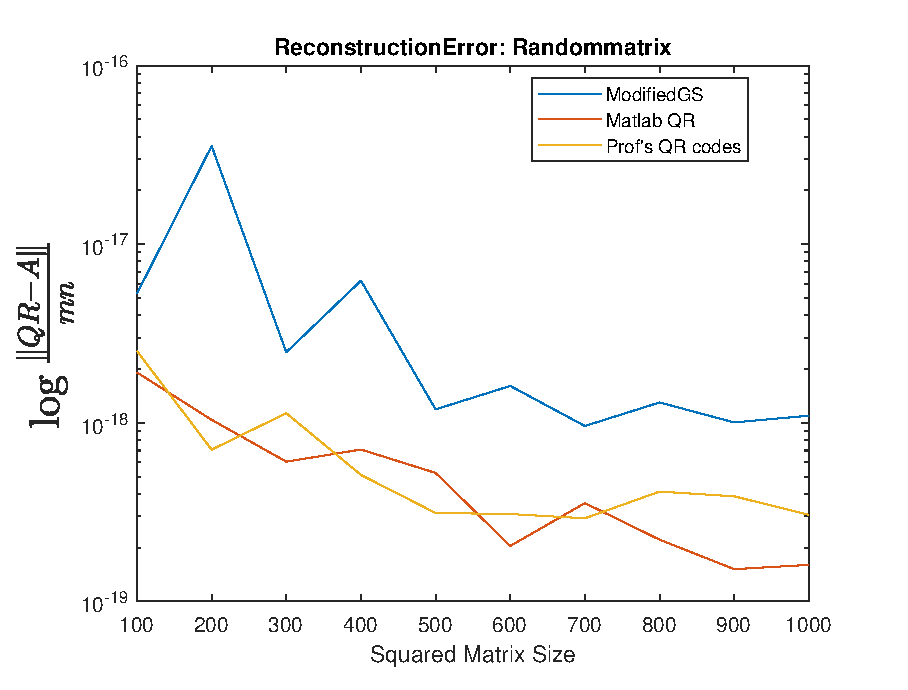
\includegraphics[width=\maxwidth{56.196688409433015em}]{figure_0.eps}
\end{center}
\begin{matlabcode}

figure;
semilogy(MatrixSizes, OrthErrs(1, :)); 
hold on;
semilogy(MatrixSizes, OrthErrs(2, :)); 
semilogy(MatrixSizes, OrthErrs(3, :)); 
title("OrthoError: Randommatrix");
legend("ModifiedGS", "Matlab QR", "Prof's QR codes", "location", "best");
xlabel("Squared Matrix Size");
ylabel("$\log{\frac{\Vert Q^HQ - I \Vert}{n^2}}$", "interpreter", "latex", "FontSize", 20);
saveas(gcf, "OrthogonalityError Randommatrix", "png");
\end{matlabcode}
\begin{center}
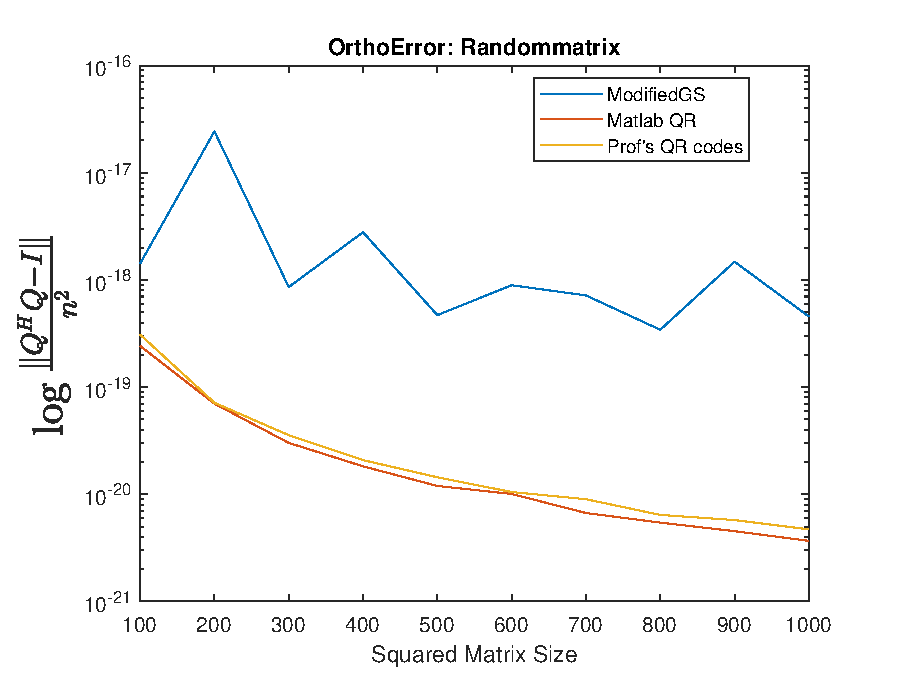
\includegraphics[width=\maxwidth{56.196688409433015em}]{figure_1.eps}
\end{center}


\matlabheadingthree{Pertubated Low Rank Matrix for accurancy testing }


\vspace{1em}
\begin{matlabcode}
import java.util.ArrayList;
Matrices = ArrayList();
MatrixSizes = 10: 100;
for I = MatrixSizes
    Matrices.add(1./(1:I)'*(1:I) + rand(I)*1e-14);
end
[OrthErrs, RestrucErrs] = PerformenceSubroutine(Matrices,{@ModifiedGS, @qr, @QRFactorFromClass});

\end{matlabcode}


\begin{matlabcode}

figure;
semilogy(MatrixSizes, RestrucErrs(1, :)); 
hold on;
semilogy(MatrixSizes, RestrucErrs(2, :)); 
semilogy(MatrixSizes, RestrucErrs(3, :)); 
title("ReconstructionError: LowRankNoisyMatrix");
legend("ModifiedGS", "Matlab QR", "Prof's QR codes", "location", "best");
xlabel("Squared Matrix Size");
ylabel("$\log{\frac{\Vert QR - A \Vert}{mn}}$", "interpreter", "latex", "FontSize", 20);
saveas(gcf, "ReconstructionError LowRankNoisyMatrix", "png");
\end{matlabcode}
\begin{center}
\includegraphics[width=\maxwidth{56.196688409433015em}]{figure_2.eps}
\end{center}
\begin{matlabcode}

figure;
semilogy(MatrixSizes, OrthErrs(1, :)); 
hold on;
semilogy(MatrixSizes, OrthErrs(2, :)); 
semilogy(MatrixSizes, OrthErrs(3, :)); 
title("OrthoError: LowRankNoisyMatrix");
legend("ModifiedGS", "Matlab QR", "Prof's QR codes", "location", "best");
xlabel("Squared Matrix Size");
ylabel("$\log{\frac{\Vert Q^HQ - I \Vert}{n^2}}$", "interpreter", "latex", "FontSize", 20);
saveas(gcf, "OrthogonalityError LowRankNoisyMatrix", "png");
\end{matlabcode}
\begin{center}
\includegraphics[width=\maxwidth{56.196688409433015em}]{figure_3.eps}
\end{center}
\begin{matlabcode}

\end{matlabcode}


\matlabheadingthree{Hilbert Matrix Accuracy Testing}

\begin{par}
\hfill \break
\end{par}

\begin{matlabcode}
import java.util.ArrayList;
Matrices = ArrayList();
MatrixSizes = 10: 100;
for I = MatrixSizes
    [X, Y] = meshgrid(1:I);
    HilbertMatrix = 1./(X + Y);
    Matrices.add(HilbertMatrix);
end
[OrthErrs, RestrucErrs] = PerformenceSubroutine(Matrices,{@ModifiedGS, @qr, @QRFactorFromClass});
\end{matlabcode}


\begin{par}
\begin{flushleft}
Plotting all of them out: 
\end{flushleft}
\end{par}


\vspace{1em}
\begin{matlabcode}
figure;
semilogy(MatrixSizes, RestrucErrs(1, :)); 
hold on;
semilogy(MatrixSizes, RestrucErrs(2, :)); 
semilogy(MatrixSizes, RestrucErrs(3, :)); 
title("ReconstructionError: HilberMatrix");
legend("ModifiedGS", "Matlab QR", "Prof's QR codes", "location", "best");
xlabel("Squared Matrix Size");
ylabel("$\log{\frac{\Vert QR - A \Vert}{mn}}$", "interpreter", "latex", "FontSize", 20);
saveas(gcf, "ReconstructionError HilberMatrix", "png");
\end{matlabcode}
\begin{center}
\includegraphics[width=\maxwidth{56.196688409433015em}]{figure_4.eps}
\end{center}
\begin{matlabcode}

figure;
semilogy(MatrixSizes, OrthErrs(1, :)); 
hold on;
semilogy(MatrixSizes, OrthErrs(2, :)); 
semilogy(MatrixSizes, OrthErrs(3, :)); 
title("OrthoError: HilberMatrix");
legend("ModifiedGS", "Matlab QR", "Prof's QR codes", "location", "best");
xlabel("Squared Matrix Size");
ylabel("$\log{\frac{\Vert Q^HQ - I \Vert}{n^2}}$", "interpreter", "latex", "FontSize", 20);
saveas(gcf, "OrthogonalityError HilberMatrix", "png");
\end{matlabcode}
\begin{center}
\includegraphics[width=\maxwidth{56.196688409433015em}]{figure_5.eps}
\end{center}
\begin{matlabcode}



\end{matlabcode}


\matlabheadingthree{Vandermonde Matrix Accuracy Testing}

\begin{par}
\hfill \break
\end{par}

\begin{matlabcode}
import java.util.ArrayList;
Matrices = ArrayList();
MatrixSizes = 10: 100;
for I = MatrixSizes
    Matrices.add(vander(linspace(-2, 2, I)));
end
[OrthErrs, RestrucErrs] = PerformenceSubroutine(Matrices,{@ModifiedGS, @qr, @QRFactorFromClass});
\end{matlabcode}


\begin{par}
\begin{flushleft}
Plotting things out: 
\end{flushleft}
\end{par}

\begin{matlabcode}
figure;
semilogy(MatrixSizes, RestrucErrs(1, :)); 
hold on;
semilogy(MatrixSizes, RestrucErrs(2, :)); 
semilogy(MatrixSizes, RestrucErrs(3, :)); 
title("ReconstructionError: Vandermonde");
legend("ModifiedGS", "Matlab QR", "Prof's QR codes", "location", "best");
xlabel("Squared Matrix Size");
ylabel("$\log{\frac{\Vert QR - A \Vert}{mn}}$", "interpreter", "latex", "FontSize", 20);
saveas(gcf, "ReconstructionError Vandermonde", "png");
\end{matlabcode}
\begin{center}
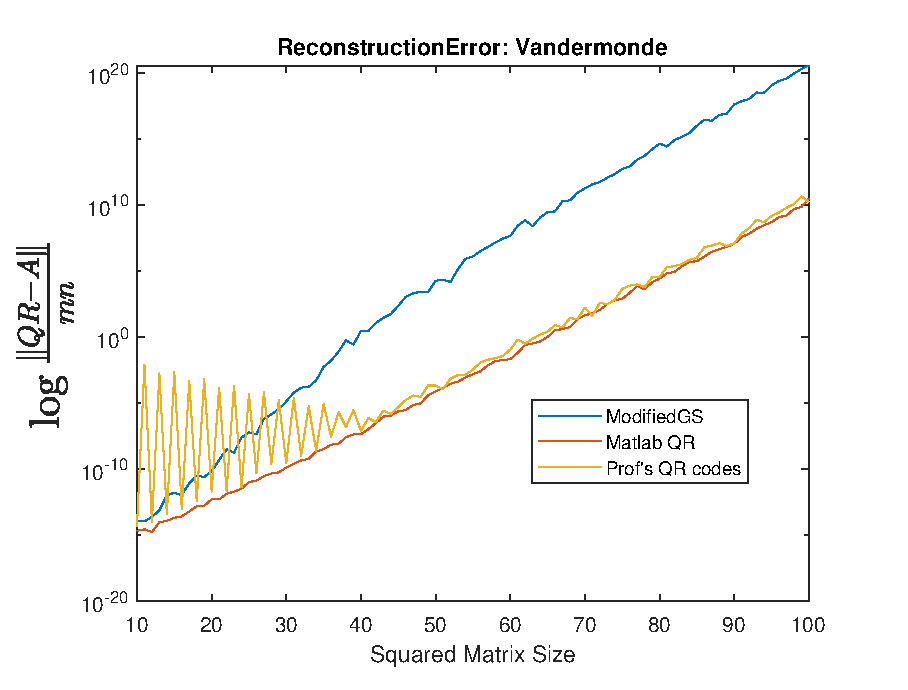
\includegraphics[width=\maxwidth{56.196688409433015em}]{figure_6.eps}
\end{center}
\begin{matlabcode}

figure;
semilogy(MatrixSizes, OrthErrs(1, :)); 
hold on;
semilogy(MatrixSizes, OrthErrs(2, :)); 
semilogy(MatrixSizes, OrthErrs(3, :)); 
title("OrthoError: Vandermonde");
legend("ModifiedGS", "Matlab QR", "Prof's QR codes", "location", "best");
xlabel("Squared Matrix Size");
ylabel("$\log{\frac{\Vert Q^HQ - I \Vert}{n^2}}$", "interpreter", "latex", "FontSize", 20);
saveas(gcf, "OrthogonalityError Vandermonde", "png");
\end{matlabcode}
\begin{center}
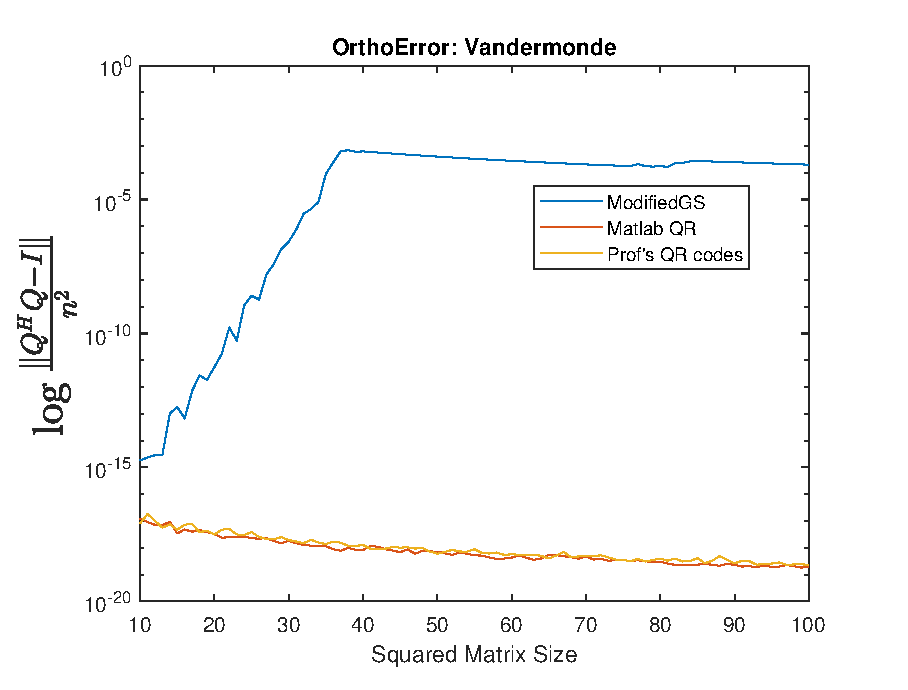
\includegraphics[width=\maxwidth{56.196688409433015em}]{figure_7.eps}
\end{center}


\matlabheadingtwo{Polynomials Conditioning}

\begin{par}
\begin{flushleft}
II (a), Plotting the badly conditioned polynomials: 
\end{flushleft}
\end{par}

\begin{matlabcode}
Xs = 1.920: 0.001: 2.08; 
plot(Xs, BadPolynomial(Xs))
saveas(gcf, "BadPolynomial.png", "png")
\end{matlabcode}


\vspace{1em}
\begin{par}
\begin{flushleft}
II (b), Plotting the goodly conditioned polynomials: 
\end{flushleft}
\end{par}

\begin{matlabcode}
Xs = 1.920: 0.001: 2.08; 
plot(Xs, GoodPolynomial(Xs))
saveas(gcf, "GoodPolynomial.png", "png")
\end{matlabcode}


\matlabheadingtwo{Matrix Conditioning}


\vspace{1em}
\begin{par}
\begin{flushleft}
Condition number of a random matrix as the size increases. 
\end{flushleft}
\end{par}


\vspace{1em}
\begin{matlabcode}
MatrixSizes = 1:10:1000
ConditionNumbers = zeros(1, length(MatrixSizes))
for I = length(MatrixSizes)
    ConditionNumbers(I) = cond(rand(MatrixSizes(I)));
end

\end{matlabcode}


\begin{par}
\begin{flushleft}
Plotting it out: 
\end{flushleft}
\end{par}

\begin{matlabcode}


\end{matlabcode}

\end{document}
